%%%%%%%%%%%%%%%%%%%%%%%%%%%%%%%%%%%%%%%%%%%%%%%%%
\section{Topology of books of \texorpdfstring{$I$}{I}-bundles}
%%%%%%%%%%%%%%%%%%%%%%%%%%%%%%%%%%%%%%%%%%%%%%%%%

In this section we establish basic definitions and facts about books of
$I$-bundles and quasi-Fuchsian surfaces contained inside them. While the
detailed arguments are new, these are basic applications of standard
``cut-and-paste'' techniques in $3$-manifold topology. See Hempel \cite{He} or
Jaco \cite{Ja}. Schultens \cite{Sch} is a gentler treatment.

Recall that we are considering possible pared structures $P$ on $M$ a convex
hyperbolic $3$-manifold. Our goal is to find a surface map $\phi \colon S \to
M$ that is quasi-Fuchsian --- ie such that $S$ is a closed surface, $\phi$ is
$\pi_1$-injective, and $\pi_1P_k \cap \phi_*(\pi_1S) = 1$ for each component
$P_k$ of $P$.

Note that since we haven't fixed a basepoint, these subgroups are really only
defined up to conjugacy (that is, they're sets of free homotopy classes) ---
what we're saying is they fail to intersect for an arbitrary choice of
conjugacy class for each subgroup. This corresponds to multiples of the
parabolic curves not being freely homotopic into the immersed image of the
given surface.

\begin{defn}\label{D:boib}

An \emph{$I$-bundle} is a fiber bundle with fiber $I=[0,1]$, and base space
a compact surface with boundary. We'll refer to this as its \emph{base
surface}.  In this paper we adopt the convention that all $I$-bundles are
oriented.  The boundary of an $I$-bundle $I \to B \to \Si$ decomposes into the
\emph{binding boundary} $\pi^{-1}(\bd \Si)$ and the \emph{side boundary}
$\bigcup \bd \pi^{-1}(x)$. Note that the binding boundary is a collection of
disjoint annuli. The reason for these terms is the following definition.

A \emph{book of $I$-bundles} is a $3$-manifold obtained from the following
construction. Let $\cB$ be a collection of $I$-bundles, and $\cC$ a collection
of solid tori. Attach the $I$-bundles to the solid tori by attaching some (or
all) of the binding boundary components to disjoint nontrivial annuli in the
boundaries of the solid tori.  If we let $\cA$ be the union of glued annuli in
the resulting manifold, our manifold can be written as $M=\cB \cup_\cA \cC$.
Note that by construction each component of $\cA$ is properly embedded and
2-sided in $M$. See Figure~\ref{F:boibdef} for an example of this construction.
Figure~\ref{F:book2} illustrates the gluing map at the bottom of this diagram.

\myfig{fig-boibdef}{F:boibdef}{Constructing a book of $I$-bundles}

\myfig{fig-book2}{F:book2}{Gluing to a complicated annulus}

In this paper we additionally impose the following conditions on a book of
$I$-bundles, to avoid elementary or degenerate cases.

\begin{enumerate}

\item The underlying manifold is a compact connected orientable irreducible
hyperbolic $3$-manifold with incompressible boundary.

\item Each page is an $I$-bundle over a surface of negative Euler
characteristic.

\end{enumerate}

\end{defn}

This is a standard definition. See papers of Culler--Shalen \cite[pp286]{CS}
and Agol--Culler--Shalen \cite[Definition 2.1]{ACS} for the original definition
and previous study of this special class of hyperbolic $3$-manifolds.

Intuitively, if we take a physical book with thick pages and imagine bending it
in a circle so its top and bottom are identified, the spine becomes a solid
torus.  If we also attach each page along its top and bottom, the pages become
thickened annuli, attached to the spine at one end. This manifold can be built
from the above construction. Take $\cC$ to be a single solid torus, and $\cB$
to be a union of thickened annuli, one for each page of the book. Glue one
gluing annulus of each component of $\cB$, and glue them all to parallel
longitudinal annuli in $\bd \cC$.

\begin{defn}

In keeping with the ``book'' terminology, we will generally refer to the
components of $\cB$ as \emph{pages}, the components of $\cC$ as \emph{spines},
and the components of $\cA$ as \emph{bindings} or \emph{binding annuli}.
Furthermore, we'll say that $M$ is \emph{fully bound} if all binding boundary
components of all pages are glued, that is, correspond to binding annuli in
$M$.

\end{defn}

See Figures~\ref{F:page} and \ref{F:spine} for illustrations of a prototypical
page and spine.

% hax: two figures side by side. Captions line up by manually adjusting!
\begin{figure}
\noindent
    \begin{minipage}{0.45\textwidth}
        \noindent
        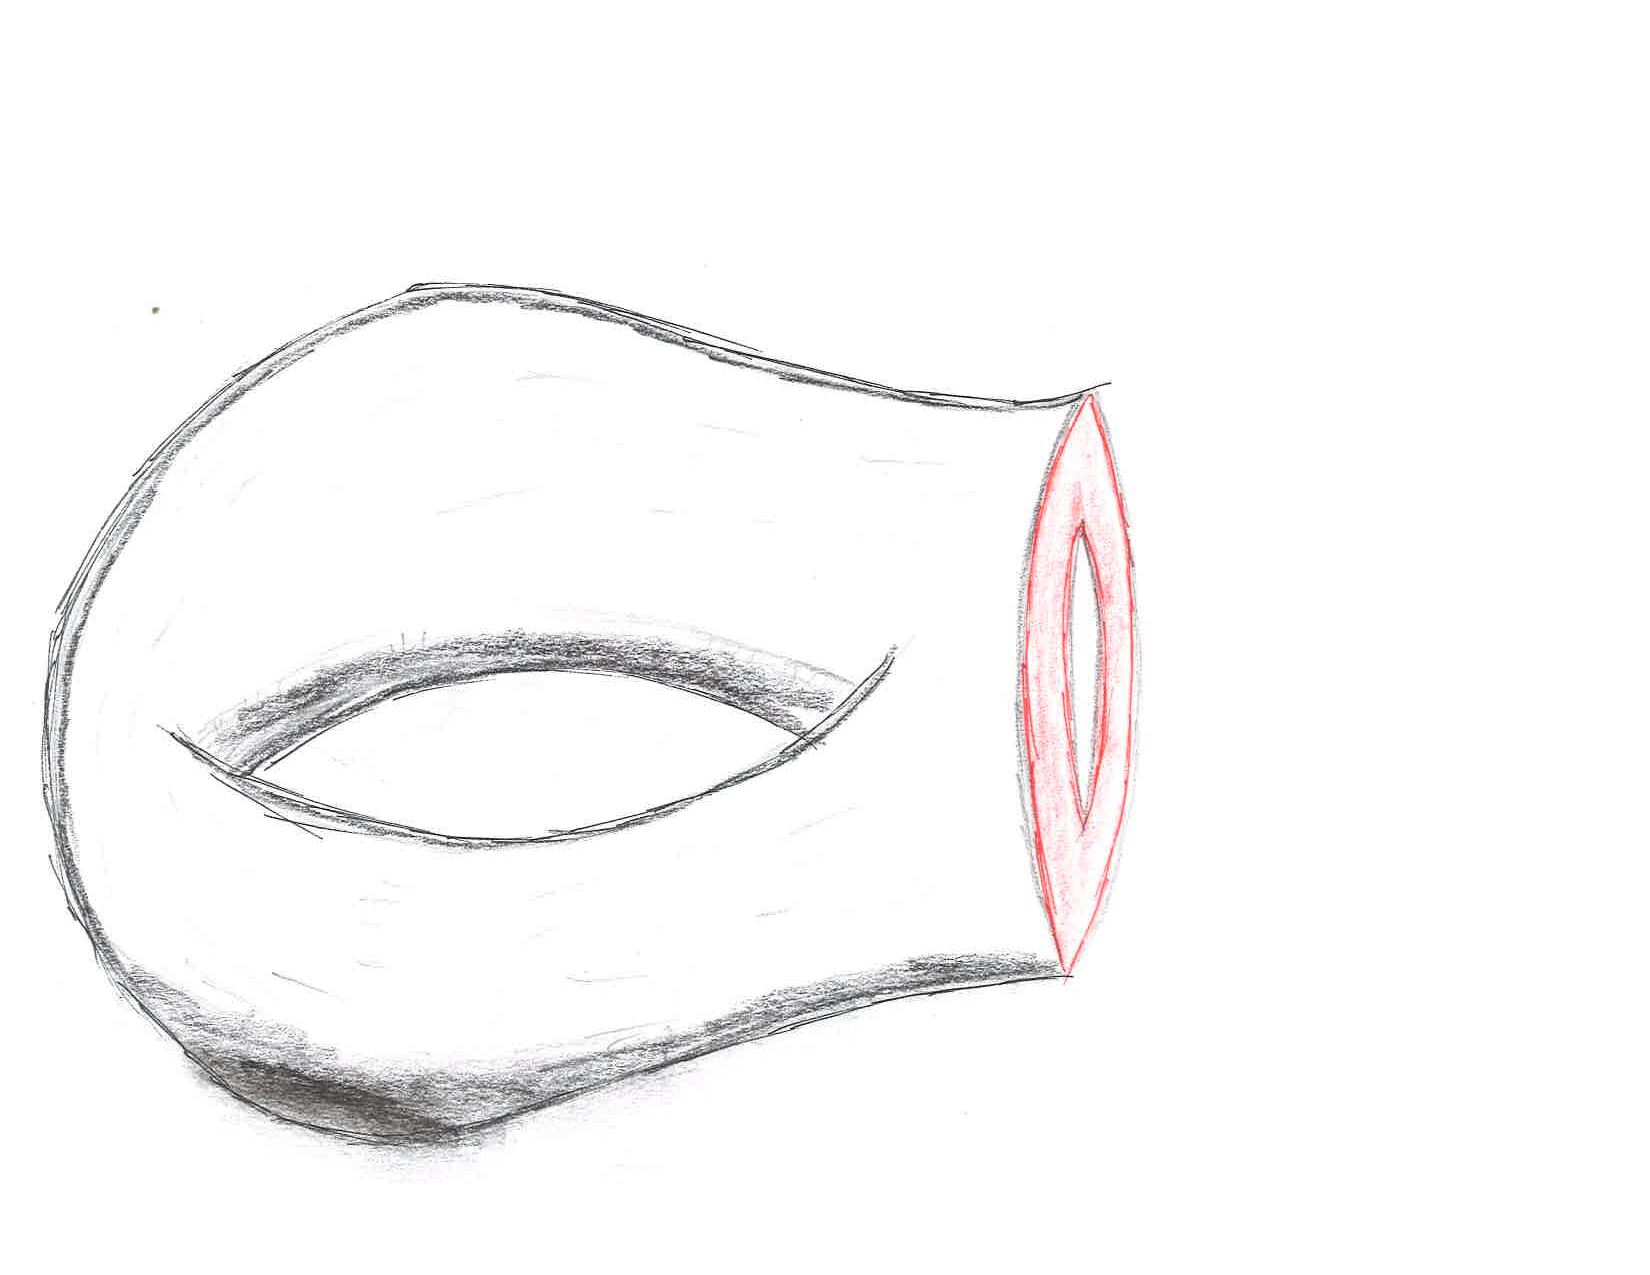
\includegraphics[width=\textwidth,height=2in]{fig-page}
        \caption{Page with one gluing annulus}
        \label{F:page}
    \end{minipage}\hfill
    \begin{minipage}{0.45\textwidth}
        \noindent
        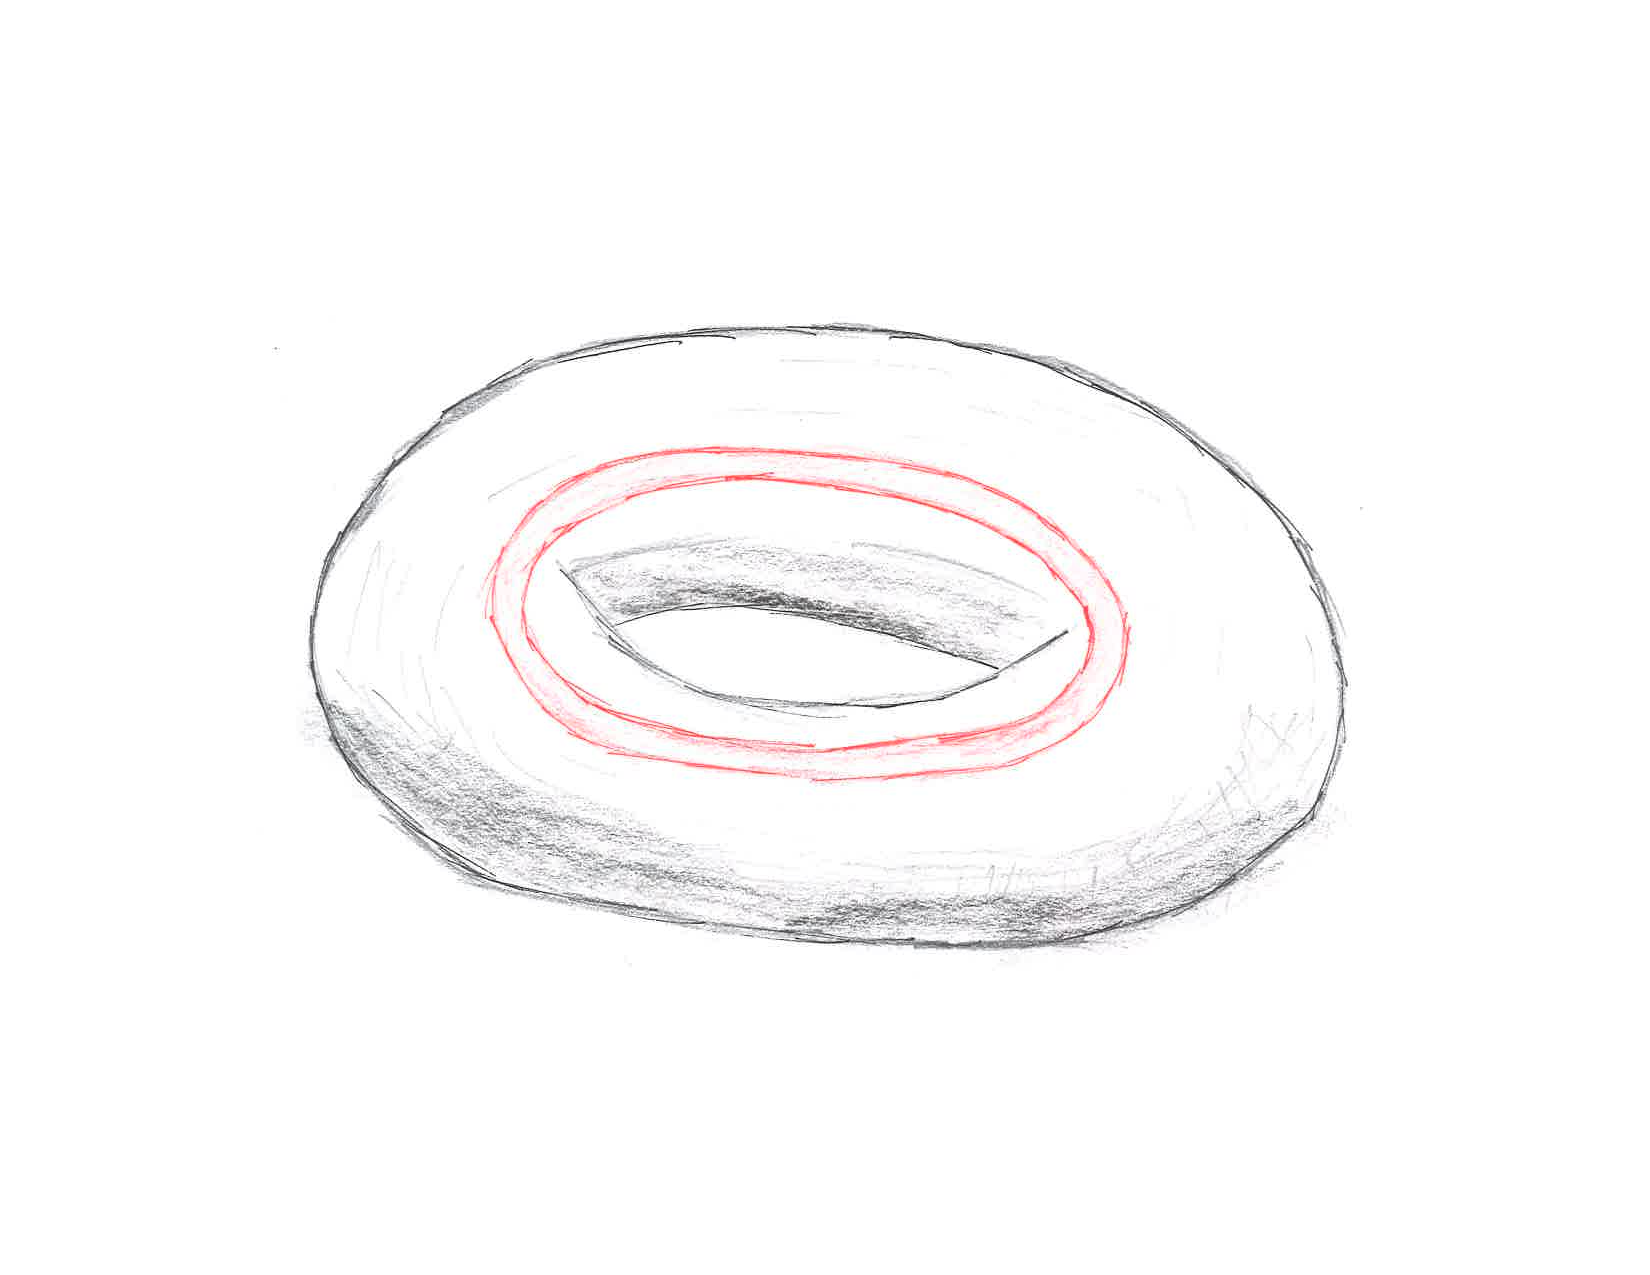
\includegraphics[width=\textwidth,height=2.05in]{fig-spine}
        \caption{Spine with one gluing annulus}
        \label{F:spine}
    \end{minipage}
\end{figure}

For reasons we'll see later, the books of $I$-bundles that we want to consider
should all be fully bound.

Algebraically, a book of $I$-bundles corresponds to a particularly simple graph
of groups. The graph is bipartite, and one side of the partition (the spines)
are just copies of $\bZ$. The other side has noncyclic free groups,
corresponding to surfaces of negative Euler characteristic. The edge groups are
copies of $\bZ$ as well.

Let's briefly explain why we impose the two conditions in
Definition~\ref{D:boib}.  Obviously we want $M$ to be compact connected
orientable hyperbolic, as this is the general case we're studying (Kleinian
manifolds). If $M$ were nonorientable we could reduce to the orientable double
cover. Hyperbolic $3$-manifolds must be irreducible.

If $M$ had compressible boundary, let $D$ be a compressing disk for the
boundary.  Consider a $\pi_1$-injective closed surface map $\phi \colon S \to
M$ whose image intersects $D$. The preimage $\phi^{-1}(D)$ is a union of simple
closed curves in $S$, since $D$ is properly embedded.  Every such closed curve
$\alpha$ has homotopically trivial image in $M$, because it's a curve in the
disk $D$.  But $S$ is $\pi_1$-injective, so $\alpha$ must be homotopically
trivial in $S$ as well.  Since $S$ is a surface, contracting the loop $\alpha$
yields a disk $D'\cin S$. Combining $\phi(D')$ and a contraction for
$\phi(\alpha)$ in $D$ yields a sphere map $S^2 \to M$. $M$ is irreducible,
hence aspherical, so this map is homotopically trivial. Using one hemisphere of
this homotopy, we can homotope $\phi(D')$ across $D$ to remove the intersection
curve $\phi(\alpha)$. Repeating this process, we can assume that $\phi(S)$ is
disjoint from $D$. This proves that any quasi-Fuchsian surfaces are essentially
disjoint from compression disks.  Therefore, since we're interested in
quasi-Fuchsian surfaces, we might as well compress as much as possible before
looking for surfaces. This also follows from the similar discussion in Chapter
3.

Ignoring for the moment the degenerate case of a single page and no spine, each
page's base surface must have at least one boundary component to glue to in
order for $M$ to be connected. We don't want to consider base surfaces which
are disks.  Observe that each page which is a disk means that that page and its
attached spine form a $3$-manifold with a finite-sheeted cover by
a $k$-puctured ball --- that is, a cover of a punctured lens space. This is
because we can arrange things so that in the cover, the disk attaching map only
traverses the longitude once, and we get a thickened disk.  This means that
we'll have finite order summands in our group, which correspond to elliptic
pieces, for instance lens spaces, in the JSJ decomposition. These cases are not
hyperbolic.

Similarly, allowing annulus or Moebius strip base surfaces means that many
books of $I$-bundles we build will not be hyperbolic. For instance, by chaining
annulus pages together in a loop, we can construct a book of $I$-bundles
containing a closed non-peripheral immersed torus. In fact, in any case where
there are no such loops, we can homotope away all the annulus pages (attaching
the associated spines together, and possibly passing to a finite sheeted
cover).  The case of Moebius strips is identical once we pass to a double cover
on each Moebius strip page. Therefore we will not consider these in the sequel.

Finally, our definition does technically allow for $M$ to consist of a single
page and no spines. Since $M$ is connected, this is the only case where $M$ can
contain a page with closed base surface. In this case, the page's base surface
obviously must have negative Euler characteristic in order for $M$ to be
nonelementary hyperbolic. (Note that a thickened torus is realized by
a Kleinian group, but this group must be elementary). Combining all these
cases, we only want to consider base surfaces with negative Euler
characteristic.

We make the following simple observation.

\begin{prop}

Let $M$ be a book of $I$-bundles, and $M'$ to $M$ be a finite-sheeted covering
space.  Then $M'$ is also a book of $I$-bundles.

\end{prop}

\begin{proof}

This is straightforward. Lift the spines and pages of $M$ to obtain spines and
pages of $M'$. Lift the gluing annuli of $M$ to gluing annuli of $M'$.

\end{proof}

These facts are well-known basic results in $3$-manifold topology.  The
following result follows immediately from the classification of $I$-bundles
over surfaces.

\begin{prop}

Let M be a book of $I$-bundles. Recall we require that $M$ is oriented. To be
orientable, every $I$-bundle in $M$ is either a trivial bundle over an oriented
surface, or a $\bZ/2$-twisted bundle over a nonorientable surface. In the
latter case, the homotopy classes in the base with nontrivial bundle twisting
are precisely those without a consistent tubular neighborhood orientation.

Furthermore, every twisted $I$-bundle has a double cover which is a trivial
$I$-bundle over a base surface which is an oriented double cover of the
original nonorientable base surface.

\end{prop}

\begin{proof}

See Hempel \cite[Theorem 10.5]{He}.

\end{proof}

This fact reflects the origin of the book of $I$-bundles construction from
a relative JSJ decomposition.

To analyze the boundary components of a book of $I$-bundles, we'll need
a couple more simple definitions.

\begin{defn}

Let $M$ be a book of $I$-bundles, and $C$ a spine in $M$.  The \emph{valence}
$v(C)$ is the number of binding annuli that intersect $C$ or, equivalently,
that are contained in $\bd C$.

Let $A$ be a binding annulus in $M$. Note that $A$ lies in the boundary of
exactly one spine $C_A$. The \emph{degree} of $A$ is the geometric intersection
number $i(A,D)$, where $D$ is a meridian disk of $C_A$. That is, it's the
minimal number of components of $A \cap D$ as we properly isotope $D \cin C_A$
and $A \cin \bd C_A$.

In fact, note that all binding annuli in a given spine $C$ must have the same
degree. This is because their core curves are curves on a torus, and any
nontrivial curves with different slopes must intersect. However, by definition
binding annuli are disjoint. Since they have the same slope, they intersect
a meridian curve (slope $\infty$) the same number of times.  Therefore, we
refer to this as the \emph{degree} $d(C)$ of the spine $C$.

\end{defn}

\begin{prop}\label{P:1ptcap}

Let $M$ be a book of $I$-bundles. Recall that we require that $M$ has
incompressible boundary. Then $M$ cannot have any spines $C$ such that
$v(C)=0$, $d(C)=0$, or $v(C)=d(C)=1$. Furthermore, $M$ must be fully glued ---
that is, it cannot have any leftover binding annuli of pages that are not
attached to spines.

\end{prop}

\begin{proof}

Any spine $C$ with $v(C)=0$ forces $C$ to be a solid torus component. This does
not have incompressible boundary (it also cannot be nonelementary hyperbolic).

Any spine $C$ with $d(C)=0$ has a meridian disk that properly embeds in the
resulting book of $I$-bundles, since it's disjoint from all the binding annuli.
This is a boundary compressing disk.

% The following case is my old nemesis, the ``one-point intersection lemma''

Let $C$ be a spine with $v(C)=d(C)=1$. Let $A$ be the sole binding annulus, $B$
the attached page, and $\Si$ its base surface. Let $\beta$ be the projection of
$A$ down to $\Si$. $\beta$ is a boundary component of $\Si$. Let $\alpha$ be an
essential arc in $\Si$ with both (distinct) endpoints in $\beta$. Note that
such an $\alpha$ must exist as $\Si$ has negative Euler characteristic. The
preimage of $\alpha$ under the projection is a rectangle $R \cin B$ with two
edges $\gamma_1$,$\gamma_2$ in the the side boundary of $B$, and two edges
$\delta_1$,$\delta_2$ that are parallel proper essential arcs in $A$. See
Figure~\ref{F:1ptcap}. Since $A$ intersects each meridian disk of $C$ exactly
once, and does so in a single essential arc, we can construct two meridian
disks $D_1$, $D_2$ such that $D_1 \cap R = \delta_1$, and $D_2 \cap
R = \delta_2$.  Let $D = D_1 \cup_{\delta_1} R \cup_{\delta_2} D_2$.

We claim that $D$ is a compression disk for $\bd M$. It is properly embedded:
$D_1$ and $D_2$ are properly embedded in $C$, $R$ is properly embedded in $B$,
and the union lines up the boundary components along $A$. It suffices to show
that $\bd D$ does not bound a disk in $\bd M$. The options for such a disk $D'$
are very limited.  $C \cap \bd M$ is an annulus, and $\bd D$ divides it into
two disk regions. $D' \cap C$ must be one of these two regions, which implies
it intersects $\bd A$ in two parallel boundary arcs, each with one endpoint in
$\delta_1$ and one in $\delta_2$.  Call these arcs $\epsilon_1$ and
$\epsilon_2$.  But now we can see that the only way to bound a disk in $\bd M$
is if $\gamma_1 \cup \epsilon_1$ and $\gamma_2 \cup \epsilon_2$ bounded a disk.
But if this disk were inside $B$, either of these would project down to $\Si$
to contradict the assumption that $\alpha$ was essential. $\bd D \cin B \cup
C$, so if $D'$ essentially intersected any other spine or page it would have to
do so in an innermost disk. But $D' \cin \bd M$, so it can only essentially
intersect a page in a surface of negative Euler characteristic and a spine in
an annulus. So this is impossible, and $D'$ cannot intersect any spines or
pages outside of $B$ and $C$. This proves that $D$ is a compression disk.

Any leftover (un-glued) binding annulus on a page induces a compression disk as
well. Let $B$ be a page with base surface $\Si$ and $A$ a binding annulus in
$\bd B$ which is not glued. That is, $A \cin \bd M$. $A$ corresponds to
a boundary curve $\beta \cin \Si$. Choose a proper essential arc $\alpha \cin
\Si$ with both endpoints in $\beta$. The preimage of $\alpha$ under the bundle
map is a properly embedded disk $D \cin M$. We claim that $D$ is a compression
disk. To see this, observe that any boundary disk $D' \cin B \cap \bd M$ would
contradict that $\alpha$ was essential, by the same argument as above. $D'$
cannot intersect any other pages or spines for the same reason as well. This
proves that $D$ is a compression disk, completing the proof.

\end{proof}

\myrotfig{fig-1ptcap}{F:1ptcap}{Proof of Proposition~\ref{P:1ptcap}}

We make a few observations about the boundary of $M$. Each page contributes two
(if it's a trivial $I$-bundle) or one (if it's a twisted $I$-bundle) side
boundary pieces to the boundary of $M$. Each spine contributes a number of
disjoint annuli equal to its valence, that is, the number of attached pages.
These are the annuli in its boundary which lie in between the binding annuli.
As these glue up to form the boundary components of $M$, each spine annulus
connects two side boundaries of "adjacently glued" pages. This intuitive
picture will be very important later as we construct quasi-Fuchsian surfaces.

The following basic property will be useful later.

\begin{prop}\label{P:pagespineII}

Let $X$ be a page or spine in a book of $I$-bundles $M$. Then $X$ is
irreducible, and each binding annulus in $\bd X$ (ie component of $\cA \cap X$)
is incompressible in $X$.

\end{prop}

\begin{proof}

We first claim $\pi_2X = 0$. A trivial $I$-bundle is a thickened surface of
negative Euler characteristic, hence is aspherical. A twisted $I$-bundle has
a double cover which is a trivial $I$-bundle over the oriented double cover of
the base surface. Solid tori are aspherical as well. It follows from the sphere
theorem that $X$ is irreducible.

Let $A \cin \bd X$ be a binding annulus. To prove $A$ is incompressible in $X$,
we'll show that it is $\pi_1$-injective. Let $X$ be a solid torus. Then since
$A$ intersects a meridian disk at least once (as shown above), it must contain
a multiple of a generator of $\pi_1X$. So $A$ is $\pi_1$-injective. Let $X$ be
an $I$-bundle. Again, we can pass to a double cover which is a trivial
$I$-bundle.  Now $A \cin X$ is $\pi_1$-injective because it's a thickening of
a boundary component of a compact surface. This completes the proof.

\end{proof}

In fact, we can extend this to a few key facts for the entire book of
$I$-bundles. First, we have the following proposition:

\begin{prop}\label{P:boibincomp}

Every book of $I$-bundles that we construct without violating
Proposition~\ref{P:1ptcap} does in fact have incompressible boundary. (That is,
our definitions are consistent).

\end{prop}

\begin{proof}

Let $M$ be a book of $I$-bundles constructed without violating
Proposition~\ref{P:1ptcap}. Suppose it has compressible boundary, and let $D$
be a compression disk. $D$ is properly embedded in $M$, so it intersects the
binding annuli $\cA$ in a disjoint union of properly embedded arcs and simple
closed curves.  We first claim that we can isotope $D$ rel boundary to remove
all intersections that are closed curves.

Let $A$ be a binding annulus. Any closed curve in $A$ is either homotopic to
the core or bounds a disk in $A$. If $D$ intersects $A$ in a curve homotopic to
the core, that curve has to bound a subdisk $D' \cin D$. $D'$ is a compression
disk of $A \cin M$. We claim that such a disk must be trivial --- that is, $A$
is incompressible in $M$.  Look at $D' \cap \cA$, which is a disjoint union of
simple closed curves in $D'$, and consider an innermost curve $\alpha$ in $D'$.
$\alpha$ lies in some annulus $A' \cin \cA$.  By
Proposition~\ref{P:pagespineII}, $A'$ is incompressible in the page and spine
on each side. But since $\alpha$ is innermost, it bounds a subdisk $D'_\alpha$
of $D'$ that's contained in a single page or spine $X$. By incompressibility,
$\alpha$ must bound a disk $D''_\alpha$ in $A'$. By irreducibility, $D'_\alpha
\cup D''_\alpha$ bounds a ball in $X$, and we can isotope across this ball to
remove the intersection curve $\alpha$. Repeating this process, $D'$ cannot
intersect $\cA$ anywhere except on its boundary. But this implies that $D'$
lies in a single page or spine.  Therefore by Proposition~\ref{P:pagespineII}
$D'$ must be trivial.  Hence $A$ is incompressible in $M$, and no core curve
intersections are possible.

We have shown that $D$ can only intersect a binding annulus in curves that
bound disks in that annulus.  We now isotope $D$ rel boundary to remove all
such intersections.  Take an innermost curve $\alpha$ in $D \cap \cA$, and say
it lies in some binding annulus $A$. Since it's innermost, $\alpha$ bounds
a subdisk $D'_\alpha$ of $D$ that is properly embedded in a single page or
spine of $M$. But $\alpha$ also bounds a disk $D''_\alpha \cin A$. By
irreducibility, $D'_\alpha \cup D''_\alpha$ bounds a ball in $X$, and we can
isotope across this ball to remove the intersection curve $\alpha$. Repeating
this process, $D \cap \cA$ contains no closed curves.

Let $A$ be a binding annulus. Any properly embedded arc in $A$ is homotopic to
a standard transverse arc. If $D$ intersects $A$ in such an arc, that arc cuts
off a subdisk $D' \cin D$. $D'$ is a boundary compression disk of $A \cin M$.
As above, we claim that such a disk must be trivial --- that is, $A$ is
boundary incompressible in $M$.  We make a similar argument. Look at $D' \cap
\cA$, which is a disjoint union of properly embedded arcs in $D'$, and consider
an outermost arc $\alpha$ in $D'$.  $\alpha$ is a transverse arc of some
annulus $A' \cin \cA$. $\alpha$ cobounds a disk $D'_\alpha$ with an arc $\beta
\cin \bd D'$.  Since $\alpha$ is outermost, $D'_\alpha$ must be contained in
a single page or spine $X$ adjacent to $A'$. Note that $\beta \cin X \cap \bd
M$, and the two endpoints of $\beta$ lie on the two boundary curves of $A'$.

But if $X$ is a spine, it must have $d(X)>1$ or $v(X)>1$. Either way it is
impossible to construct such a $\beta$ connecting the endpoints of
a transversal $\alpha$ such that $\alpha \cup \beta$ bounds a nontrivial disk.
The only nontrivial embedded disk is a meridian disk, and if we try to bound
that, $\beta$ will cross a different binding annulus (if $v(X)>1$) or
a different part of the same binding annulus (if $d(X)>1$).

If $X$ is a page, it must be fully glued. Therefore, if $X$ is a trivial
$I$-bundle, $X \cap \bd M$ has two components. The two endpoints of $\alpha$
lie in two different components, so an arc $\beta \cin X \cap \bd M$ connecting
them obviously cannot exist. If $X$ is a twisted $I$-bundle, the same argument
applies after lifting to a trivial $I$-bundle double cover.

Hence any such disk $D'$ is trivial, and $A$ is boundary incompressible. Since
any such transverse arc in $D \cap \cA$ corresponds to a trivial boundary
compressing disk, we can isotope $D$ such that the intersection contains no
transverse arcs as well. But this implies that $D$ is disjoint from $\cA$.
Hence $D$ is contained in a single page or spine $X$, and $\bd D$ avoids all
the binding annuli adjacent to $X$.  Also, $\bd D$ is contained in a single
component of $X \cap \bd M$. To prove $D$ is a trivial compressing disk, we
show that the components of $X \cap \bd M$ map $\pi_1$-injectively to $X$.

If $X$ is a spine, the components of $X \cap \bd M$ are parallel to the binding
annuli, so the proof is identical to the proof of
Proposition~\ref{P:pagespineII}. If $X$ is a page, since it's fully glued, the
components of $X \cap \bd M$ are either two disjoint copies of the base surface
or an oriented double cover of the base surface. In either case they
immediately map in $\pi_1$-injectively. This proves that $X \cap \bd M$ is
incompressible in $X$.  Since $D$ is a compression disk of $X \cap \bd M$ in
$X$, it must be trivial. This completes the proof.

\end{proof}

We highlight the key facts we've proven about the binding annuli.

\begin{cor}

Let $M$ be a book of $I$-bundles. Then in fact all the binding annuli of $M$
are incompressible and boundary incompressible in $M$.

\end{cor}

We now discuss the possible closed $\pi_1$-injective surfaces inside a book of
$I$-bundles. These are the surfaces we'll need to consider in order to find
a closed quasi-Fuchsian surface --- that is, a quasi-Fuchsian surface subgroup.
Recall that we refer to these as (QF) surfaces.

Note that since every hyperbolic $3$-manifold is aspherical, by elementary
obstruction theory any injective map $\pi_1S \to \pi_1M$ is induced by
a $\pi_1$-injective map $S \to M$. See discussion in Long--Reid \cite[Section
1.1]{LR}.
% on p11

Furthermore, by minimal surface theory, we can guarantee that any
$\pi_1$-injective surface in a hyperbolic $3$-manifold is homotopic to an
immersed surface.  A surface which is not immersed will contradict minimality.
This is due to Freedman, Hass, and Scott \cite{FreedmanHassScott}. See
discussion in Neumann \cite[Section 1]{Neu}.
%on p1

In what follows we'll speak only of $\pi_1$-injective surfaces, or possibly
surface subgroups. But it is important to note that in this situation those are
the same thing, and can be chosen to be immersed as well.

\begin{lemma}[Surface covering lemma]\label{L:covering}

Let $\phi\colon S \to S'$ be a proper $\pi_1$-injective map between compact
connected oriented surfaces with boundary, and suppose that $S$ is not
a 2-sphere or an annulus.  Then $\phi$ is homotopic rel boundary to
a finite-sheeted covering map.  Note that the converse holds more generally ---
that is, any finite-sheeted covering is a proper $\pi_1$-injective map.

\end{lemma}

\begin{proof}

This is originally due to Nielsen \cite{Nielsen}. See Gabai--Kazez
\cite{GabaiKazez} for a modern discussion.

\end{proof}

We now decompose $\pi_1$-injective surfaces and pared structures on a book of
$I$-bundles across the pages and spines. This is a refinement of the
decomposition properties proved in Chapter 3.

\begin{lemma}[Surface decomposition lemma]\label{L:sfcdecomp}

Let $M$ be a book of $I$-bundles, and $\phi\colon S \to M$ be
a $\pi_1$-injective map, where $S$ is a (connected) closed orientable surface.
Abusing notation, we will also refer to the image of this map as $S$. Then, we
can place $S$ in minimal position with respect to $M$ such that:

\begin{enumerate}

\item For each page $B$, $S \cap B$ is a finite-sheeted cover of the page's
base surface (that is, to be more precise, the map $S|_{\phi^{-1}(B)} \to B \to
\Si$ is a finite-sheeted cover).

\item For each spine $C$, $S \cap C$ is a union of annuli parallel to multiples
of the binding annuli in $\bd C$. The two boundary curves of each annulus lie
in different binding annuli.

\item The page covers and spine annuli are attached along curves parallel to
the multiples of the bnding annuli at each spine. That is, for each binding
annulus $A$, $S \cap A$ is a union of multiples of the core curve of $A$. All
boundary components of the page and spine intersections are attached in this
way to yield a closed surface.

\end{enumerate}

\end{lemma}

\begin{proof}

Homotope $S$ to be transverse to $\cA$, the union of all binding annuli.
Cutting S along $\cA$ decomposes it into a union of properly immersed surfaces
in each page or spine of $M$. We first move $S$ into minimal position with
respect to $\cA$.  For each page or spine $X \cin M$, $S \cap X$ is a union of
properly immersed surfaces. Consider an arbitrary component $S'$ of $S \cap X$.

If $S'$ is a disk, its boundary is an (immersed) curve in some binding annulus
$A \cin \bd X$. $\bd S'$ is contractible in $X$ as it bounds an immersed disk.
Since $A$ is incompressible, $\bd S'$ must be contractible in $A$. Combine
these two contractions to form a map $S^2 \to X$ where the equator maps along
$\bd S'$ and each hemisphere maps along one of the contractions. Since $X$ is
aspherical, this map is homotopically trivial. This yields a homotopy of $S'$
into $A$.  To keep $S$ transverse to $\cA$, we will actually homotope it
slightly past $A$ into whatever page or spine is glued to the other side of
$A$.

Now suppose that $S'$ is an annulus, and that both boundary curves of $S'$ lie
in the same binding annulus $A$. We claim that $S'$ is homotopic rel boundary
to an annulus in $A$. We know the two boundary components are conjugate in
$\pi_1$ (they're freely homotopic, following $S'$). Since they both lie in $A$,
they must be parallel, as different multiples of the generator of $\pi_1A$
cannot possibly be conjugate in $\pi_1X$ (which is cyclic or free). It follows
that they bound an annulus $S''$ in $A$.  To prove $S'$ and $S''$ are
homotopic, observe that together they describe a map $\psi\colon T^2 \to X$.
But $\pi_1X$ does not contain an abelian group of rank greater than 1, so
$\psi$ cannot be $\pi_1$-injective.  Choose a primitive $\beta$ for the kernel
of this map. $\beta$ bounds an immersed disk $D$.  Cutting $S \cup S''$ along
$\beta$ and attaching 2 parallel copies of $D$ yields a map $\psi'\colon S^2
\to X$.  But $X$ is aspherical, so this map is homotpic to a point. Following
along this homotopy (and reversing part of it) yields a homotopy between $S'$
and $S''$.

Suppose we have eliminated every piece of $S$ which is a disk or disallowed
annulus in this way, by homotoping it across the binding annuli. We may need to
repeat inductively, but at every stage we're reducing the number of
intersections with $\cA$ so this is guaranteed to terminate. We now claim that
after no more such moves can be made, the result satisfies (1) and (2).

Again consider an arbitrary page or spine $X$, and an arbitrary component $S'$
of $S \cap X$.  We know $\pi_1S' \neq 1$ by the above argument. We also know it
cannot be an annulus if $X$ is a page. Annuli with both boundary components on
the same binding annulus were removed above, and no other annuli can exist
because they'd project down to give a $\pi_1$ conjugacy between two boundary
classes in a surface with boundary, which is impossible as $\pi_1X$ is
a noncyclic free group.  We claim it is $\pi_1$-injective as a map $S' \to X$
(abusing notation slightly --- really this is asking about the preimage of $S'$
on the left-hand abstract surface $S$).  Suppose not. Then we have a nontrivial
loop $\alpha \cin S'$, which is homotopically trivial in $X$.  Therefore
$\alpha$ is homotopically trivial in $M$, using that same homotopy.  Since $S
\to M$ is $\pi_1$-injective, $\alpha$ must be homotopically trivial in $S$.
Since $S$ is an oriented surface, the only way $\alpha$ can be homotopically
trivial in $S$ but not $S'$ is if one of the boundary components of $S'$ cuts
off a disk $D \cin S$. If it cuts off a surface of any higher genus, we do not
obtain any relations among elements of $\pi_1S'$.  But if we cut $D$ along
$\cA$, we can see that at least one innermost piece of $D$ must be a disk,
contradicting our minimality assumption.  Hence each piece $S'$ is
$\pi_1$-injective in $X$.

Let $B$ be a page. We know that each piece $S'$ of $S \cap B$ is
$\pi_1$-injective and proper. Projecting $B$ to its base surface $\Si$, we know
this is a deformation retract ($B$ is an $I$-bundle) so the composition $S'$ to
$\Si$ is also $\pi_1$-injective and proper. Applying the covering lemma, we see
that each piece $S'$ is homotopic rel boundary to a finite-sheeted covering of
$\Si$.  This proves (1).

Let $C$ be a spine. Again we know that each piece $S'$ of $S \cap C$ is
$\pi_1$-injective and proper. Since $C$ has cyclic fundamental group, and no
piece $S'$ is a disk, every piece $S'$ must be an annulus. These annuli are
$\pi_1$-injective, and by construction must have boundary curves on different
binding annuli.  This proves (2).

To prove (3), look at the boundary curves of these annuli in the spines. Each
boundary curve must be contained in a binding annulus $A \cin \bd C$. Therefore
it must be a multiple of the cure curve of $A$. This proves the first statement
in (3). The remainder of (3) follows directly from the fact that $S$ is
a closed surface and that $M$ is a union of pages and spines along binding
annuli.

\end{proof}

We now consider the possible pared structures $(M,P)$, where $M$ is a book of
$I$-bundles. We have a straightforward fact.

\begin{prop}\label{P:annuli}

Let $M$ be a book of $I$-bundles, and $P$ a pared structure on $M$. $P$ cannot
contain any tori.  That is, $P$ consists entirely of annuli.

\end{prop}

\begin{proof}

Each page of $M$ has a base surface of negative Euler characteristic, so each
component of a page boundary must also have negative Euler characteristic (it's
either a copy or an orientable double cover of the base surface, as discussed
earlier). Since each boundary component of $M$ consists of page boundaries
glued together along annuli in spines, which contribute nothing to Euler
characteristic, it immediately follows that each boundary component of M has
negative Euler characteristic itself. So no boundary component admits
a $\pi_1$-injective torus, and all pared locus components must be annuli.

\end{proof}

\begin{lemma}[Pared decomposition lemma]

Let $(M,P)$ be a pared $3$-manifold, where $M$ is a book of $I$-bundles. Then we
can isotope $P$ within $\bd M$ such that:

(1) For each page $B$, $P \cap B$ is a union of disjoint rectangles and annuli,
each of which projects to a thickened arc or curve in the base surface $\Si$ of
$B$.  Any such arc or curve is essential in $\Si$.

(2) For each spine $C$, $P \cap C$ is a union of disjoint rectangles and at
most one annulus.  Each rectangle connects two adjacent binding annuli in $\bd
C$ along a thickened arc that is essential in that component of $\bd M \cap C$
(the "intermediate annulus" between these two binding annuli). The annulus
component, if any, is parallel to the binding annuli in $\bd C$.

(3) For each binding annulus $A$, $P \cap A$ is a union of disjoint arcs in
$\bd A$.

\end{lemma}

\begin{proof}

We can isotope $P$ locally, keeping all its components disjoint and embedded in
$\bd M$, so that it's transverse to $\cA$. This immediately guarantees (3).

Let $X$ be a page or spine in $M$. $P \cap X$ is a union of disjoint rectangles
and annuli, which are thickenings of arcs and curves in $\bd M \cap X$. Suppose
one of these is an arc $\alpha$ which is not essential in $\bd M \cap X$. Then
$\alpha$ cobounds a disk with an arc in $\bd (\bd M \cap X)$. There may be
other arcs in the interior of this disk, but with an innermost disk argument we
can inductively push all such arcs out of $\bd M \cap X$ while keeping them
disjoint.  Note that the interior of this disk cannot contain any closed curves
coming from $P$ because they would not be $\pi_1$-injective. This is an isotopy
of $P$ inside $\bd M$.  Repeat this inductively for all pages and spines until
no such arcs remain at all.  Since at each step we're decreasing the number of
intersections of $P$ with $\cA$, this process is guaranteed to terminate.

Let $B$ be a page. Let $\alpha$ be a closed curve in $\bd M \cap B$ which
thickens to an annulus in $P \cap B$. $\alpha$ cannot bound a disk in $\bd
M \cap B$, or that component of $P$ would fail to be $\pi_1$-injective in $\bd
M \cap B$, hence in $M$. So either $\alpha$ is essential in $\bd M \cap B$, or
$\alpha$ is parallel to a component of $\bd(\bd M \cap B)$. In the latter case,
if this component corresponds to a binding annulus $A$, push the thickened
$\alpha$ annulus across $A$ into the attached spine.  There cannot be any
annuli or rectangles in between, because components of $P$ can't be parallel
and we already eliminated all the non-essential rectangles.

Suppose we've performed the above isotopy on $P$. Since we can preserve
transversality, (3) still holds. We claim the result satisfies (1) and (2).

To prove (1), let $B$ be a page. Observe that the rectangles and annuli in $P
\cap B$ are thickenings of arcs and curves which are essential  in $\bd M \cap
B$. Let $\Si$ be the base surface of $B$. As discussed above, $\bd M \cap B$ is
either two copies of $\Si$ (if $B$ is a trivial $I$-bundle) or an orientable
double cover of $\Si$ (if B is a twisted $I$-bundle). In either case the
projection of each arc and curve must be essential in $\Si$, as otherwise we
could lift a contracting or boundary-exiting isotopy to $\bd M \cap B$. This
proves (1).

To prove (2), let $C$ be a spine. Observe that $\bd M \cap C$ is a union of
parallel annuli, each of which is parallel to the binding annuli in $\bd C$.
Rectangles in $C$ are essential, as guaranteed earlier. Up to isotopy, the only
embedded closed curve in an annulus is the core curve. So the only annuli in $P
\cap C$ are parallel to the binding annuli. Because the components of $P$ are
nonparallel in $\pi_1M$, there is at most one annulus component of $P\cap C$.
This completes the proof.

\end{proof}

\begin{defn}

Let $(M,P)$ be a pared $3$-manifold, where $M$ is a book of $I$-bundles.  We
say that $P$ is \emph{in minimal position} if it satisfies the requirements of
the pared decomposition lemma. Similarly, we say that a closed
$\pi_1$-injective immersed surface $S\cin M$ is \emph{in minimal position} if
it satisfies the requirements of the surface decomposition lemma.

\end{defn}

Let $M$ be a book of $I$-bundles, and $S \to M$ be a $\pi_1$-injective map,
where $S$ is a connected closed surface.  Place $S$ and $P$ in minimal position
as above.  We have a constructive topological criterion for when $S$ is a (QF)
surface.

Construct a "pared lifting pattern" on $S$ as follows. We build a pattern of
arcs and curves on each component of $S \cap X$, where $X$ is a spine or page.
For each page $B$, a component $S'$ of $S \cap B$ is a finite-sheeted cover of
the base surface $\Si$ of $B$. The side boundary $\bd M \cap B$ is either two
copies of $\Si$ or an oriented double cover. In either case, we have
a canonical covering map from $S'$ to each component of $\bd M \cap B$. We
define the pared lifting pattern on $S'$ to be the preimages of the projection
of $P \cap B$ to $\Si$ under these covering maps.  Note that these images may
intersect even though they are disjoint in $P \cap B$, because pushing down to
$\Si$ may cause overlaps.

For each spine $C$, a component $S'$ of $S \cap C$ is an immersed annulus
parallel to a multiple of the binding annuli.  The two components of $\bd S'$
lie on two distinct binding annuli. Now there may or may not be a component
$A'$ of $\bd M \cap C$ with boundary components in these same two binding
annuli.  (This is true when the two binding annuli are "adjacent" in $C$). If
there is, we can homotope the boundary components of $S'$ to be multiples of
the boundary components of $A'$, since they lie in the same boundary
components.  This gives us a canonical covering map from $S'$ to $A'$. Begin by
defining the pared lifting pattern on $S'$ to be the preimage of $P \cap A'$
under this map. If there is no such component $A'$, define the pared lifting
pattern to be empty.  Now, if there are any annulus components of $P \cap C$,
these must be parallel to the binding annuli and contained in a component of
$\bd M \cap C$.  Again, they have canonical preimages under the covering map
from $S'$ to that component of $\bd M \cap C$. Add these to the pared lifting
pattern for $S'$.

We now construct the pared lifting pattern on $S$ by gluing these components of
$S \cap X$ back together to form $S$. Whenever we glue, we guarantee that for
any given component of $P$ which is represented in the pared lifting patterns
on both sides, the lifted components will connect up across the gluing.
Equivalently, if we look at a tubular neighborhood $N$ of a gluing annulus $A$,
$S \cap N$ is a union of covers of the components of $N \cap \bd M$. This gives
a local description of the pared lifting pattern near each gluing annulus ---
we want to ensure that the two sides match to give this description when we
glue.  This is easy to guarantee locally as the covering degree is the same on
both sides of each gluing, so we just need to perturb topologically so the
endpoints line up.  Another way of saying this is at each gluing, we make sure
to attach lifts of pieces of the same component of $P$, and not to attach lifts
of pieces of different components of $P$.

We generally describe the pared lifting pattern using curves and arcs, not
annuli and rectangles. The topology is identical --- we can thicken within $S$
to obtain the original pared lifting pattern.

\begin{defn}

We say that $S$ satisfies the \emph{pared lifting criterion} or \emph{parabolic
lifting criterion} if the pared lifting pattern on $S$ contains no closed
curves (equivalently, closed annuli if we view them as thickened).

\end{defn}

Note that in particular, if any page or spine of $M$ contains an annulus in
$P$, any $S$ that essentially intersects this page or spine will automatically
fail the pared lifting criterion, because that will yield a closed curve in any
overlapping pieces of $S$.

\begin{theorem}[Pared/Parabolic lifting criterion]\label{T:lift}

Let $M$ be a book of $I$-bundles, and $S \to M$ be a $\pi_1$-injective map,
where $S$ is a connected closed surface.  Place $S$ and $P$ in minimal position
as above.  $S$ is a (QF) surface if and only if it satisfies the pared lifting
criterion.

\end{theorem}

\begin{proof}

One direction is straightforward. If the pared lifting pattern contains
a closed curve $\alpha$, every arc making up $\alpha$ in a page or spine must
be a lifted copy of an arc in a single component $P_0 \cin P$, because we only
attached copies that came from the same component downstairs. Therefore the
curve $\alpha$ is locally a cover a $P_0$, hence a cover of $P_0$. This
demonstrates that $S$ contains a multiple of $P_0$ up to homotopy. So $\pi_1S$
fails to avoid all conjugates of $\pi_1P_0$, and $S$ is not a (QF) surface.

Now suppose that the pared lifting pattern contains no closed curves. We claim
that $S$ is a (QF) surface. Suppose not. Let $\alpha$ be a multiple of the core
curve of a component $P_0 \cin  P$ such that $\alpha$ is freely homotopic into
$S$.  Homotope $\alpha$ into $S$. A priori $\alpha$ is no longer in minimal
position with respect to the binding annuli. As we did with $P$, we can put now
$\alpha$ into minimal position with respect to the binding annuli.  We claim
that it's possible to homotope $\alpha$ to minimal position while keeping it
within $S$.  To prove this, follow the procedure above to homotope $\alpha$ to
minimal position.  $\alpha$ begins in $S$.  Since $S$ is transverse to $\cA$,
we can obviously homotope $\alpha$ within $S$ to be transverse.  Observe that
every homotopy of a part of $\alpha$ across a disk or annulus (as in the
earlier proof of homotopy to minimal position), that same disk or annulus must
be part of the local component of $S$ that this part of $\alpha$ is contained
in.  We know this because we fully described the behavior of $S$ once we placed
it in minimal position, in the surface decomposition lemma.  $S$ will locally
cover any of the disks or annuli that we can homotope across, so the respective
parts of $\alpha$ will have available parts of $S$ to homotope within.

So we can homotope $\alpha$ to minimal position within $S$. We now claim that
we can choose this minimal position curve in $S$ to be (up to homotopy within
individual pages and spines) a multiple of the original minimal position of
$P_0$ within $(M,P)$. We know that $P_0$ began in minimal position, so any
multiple is also in minimal position. Now reverse the moves we made to homotope
$\alpha$ into $S$ originally. Because we're dividing $M$ along a union of
$\pi_1$-injective disjoint annuli, the only possible moves $\alpha$ can make
between different pages and spines are the disk and annulus moves described
above. So the reverse of our homotopy into $S$ is a homotopy toward minimal
position of the form that we described in the previous paragraph. Hence we can
perform it while keeping $\alpha$ within $S$.

This proves that $\alpha$, the multiple of $P_0$, can be homotoped to lie in
$S$, while remaining in its original minimal position with respect to the
binding annuli.  This implies that locally on each page and spine, $\alpha$ is
(up to homotopy rel boundary) some collection of multiples of the pared lifting
pattern components corresponding to $P_0$. Since any multiples connect up
between pages and spines in the same way as the original pared lifting pattern,
we find that $\alpha$ locally covers components of the pared lifting pattern.
Hence $\alpha$ covers a component of the pared lifting pattern globally.
$\alpha$ is a closed curve, so the pared lifting pattern contains a closed
curve. This completes the proof.

\end{proof}
